\documentclass[a4paper,12pt,twoside]{book}

\usepackage{pacchetti}
\usepackage{macro}
\usepackage{style}						
\usepackage[backend=biber,
		url=false,
		doi=false,
		isbn=false,
		style=alphabetic]{biblatex}    
\usepackage[toc,page]{appendix}
\usepackage{minted}
\addbibresource{bibliografia.bib}

\begin{document}  
\title{Multicriteria analysis: transportation models for value creation}																
\author{Marco Repetto \hfill}
\titolocorso{Economics and Finance}
\annoaccademico{2017/2018}
\relatore{Prof. Davide Latorre\hfill}				
\correlatore{Prof. Danilo Liuzzi\hfill}
	
	\maketitle
	\salvastmpB
	\clearpage{\pagestyle{empty}\cleardoublepage}
	\tableofcontents	
	\listoffigures		
	\listoftables	%\lstlistoflistings
	%===========================
	\clearpage{\pagestyle{empty}\cleardoublepage}
\chapter*{Introduction}
\markboth{Introduction}{Introduction}
\addcontentsline{toc}{chapter}{Introduction}

\begin{flushright}\begin{small}\textit{"There are two ways of constructing a software design;\\One way is to make it so simple that there are obviously no deficiencies.\\And the other way is to make it so complicated that there are no obvious deficiencies.\\The first method is far more difficult."}\\
Sir Charles Antony Richard Hoare\\
\end{small}\end{flushright}

\begin{doublespace}
Value and Multinational Firms are probably the pair of elements that characterized the way business was done in the last centuries. However the symbiosis behind the two is something that goes back to the begin of time, humanity and especially capitalistic societies were alwais interested in create the greatest value as possible but at the same time cutting any possible cost in order to gain extra profit from this difference.
\\
Because of this interest different disciplines were created these range from management to accounting and from supply chain to logistics; in these dissertation the scope will be to apply a multi-objective approach namely the Goal Programming in order to prove the effectiveness of such method and its different flavours in the hand of the Decision Maker. The two model presented deals with the transportation of some particular elements of the firm in order to create additional value for the firm. A firm and especially a multinational firm may be seen as a network of enterprises that intertwine between each other in order to exploit the synergies provided by such union, if the framework of logistics is used is possible to discenr the flow between two or more of such firms in three different aspects, namely:
\begin{itemize}
	\item Information: this flow consist of all the information necessary for the network to function, it maybe the information of the demand that has to move back to the production plan in order to be fullfilled;
	\item Goods: this flow is the most tangible one and may involve the movement of products from the rearline (production plan) to the frontline (retail stores);
	\item Finance: usually the finance flow is, among the information flow the one that permis the day to day operation of the network entities, this role is usually undertaken by the head quarter or in more complex groups to ad-hoc financial institution inside the multinational. 
\end{itemize}

The following dissertation will be organized into four main blocks where the first block, the introductory one, is devoted to give an overview of the notions that will be used to model the two different problems proposed in the next chapters. Chapter 1 will be a transportation model used to allocate in an efficient way different economic  components of the firm in order to achieve figgerent type of goals such as overall tax liability minimization, taking into account the regulatory requirements imposed by the international tax principles (more specifically the regulation on transfer pricing). Chapter 2 will be about Supply Chain Management and in particular Green Supply Chain Management. The aim of such model will be to fullfill the demand and the same time comply with the different regulatory legislation in terms of recycling electronical waste. Ultimately a general conclusion will be given highlithing the pro and cons of using such approach in modelling transportation problems.

\subsubsection{Multi-criteria decision analysis}
Even if the practice of decision-making is old as man, academics tend to date the roots of modern MCDA in the early 60s, where the focus at the time was to find the most preferred solution, or generating an approximation to the entire efficient frontier\cite{Greco2016}.
\\
Multi-criteria analysis may be defined as a problem of multiple-objective programming, that differs from a linear one,
since more objective function are handled; its formulation is the following:
	$$
	Min[f_1(x),f_2(x),...,f_k(x)] \quad i=1,...,k \quad where \quad k\geq2
	$$
This approach seems to fit better the real world since, in reality, more than one objective is pursued, and most of the time in contrast with one another.
A solution to a multi-criteria problem would be optimal if it'd respected the Pareto Efficient assumption, namely that no other feasible solution exists that is at least as good with respect to all objectives and strictly better with respect to at least one objective. Mathematically it means that $\left\{x_1,...x_k\right\}$ is a solution if $\not\exists \left\{x'_1,...x'_k\right\}$
such that:
	\[
	g(f_1(x),f_2(x),...,f_k(x)) \leq g(f_1(x'),f_2(x'),...,f_k(x')) \quad \forall n \quad \in  \left\{1...k\right\}
	\]
However such increase in complexity given by multiple objectives is both the strength and the weakness of such methodology, this is due to the fact that we have to deal with $N$ trade-offs deriving from the objectives we decided to include in our optimization problem. Because of this problem a lot of approaches and specific intelligent algorithms were proposed\cite{Cui2017}.

Focusing the attention on the approaches suggested, four main categories emerge, namely:

\begin{itemize}
	\item A Priori methods: such methods are characterized by prior definition of the preference information, this category includes methods such as Weighted Sum Method, Constraints Method, Objective Programming Method, Dictionary Ordering Method and Analytic Ordering Method;   
	\item Interactive methods: in this particular category the process is iterative, meaning that the decision maker interacts with the preference information he gave in search of the optimal solution, from this category belong two types of methods namely the Normal Boundary Intersection and the Normalized Normal Constraint;
	\item Pareto-dominated methods: these methods divides the optimal solution seeking in two parts, at first they try to compose the efficient frontier of a given multi-criteria problem, then they try to find the Pareto Dominant\footnote{Given a vector of outcomes $\vec{S}$ that we identified as the Efficient Frontier $\vec{S}[s_1..._n]$ a solution $s^{\star}$ of such vector is Pareto Dominant if $\nexists$ a $s_q$ that is Pareto superior to $s^{\star}$.} solution;
	\item New Dominance methods: this methods may be considered as an extension of the Pareto-dominated methods, in that they try to build the efficient frontier, then they try to eliminate the Pareto-dominated solutions however they tend to use fuzzy methods and other solutions to avoid the computational drawback of the former one.  
\end{itemize}

From the set of the A Priori methods belongs the Goal Programming (which develops from the concept of linear programming) and will be used to model the problem of entities allocation proposed on the next chapters.
\\
Goal Programming, hereinafter GP, is a multi-criteria decision analysis approach which allows the decision maker to consider simultaneously several conflicting objectives.

The idea behind such method is very simple, and is based on distance minimization; this means that at each objective function is associated a deviation variable that has to be minimized in batch with the other deviation variables coming from the other objective functions.

Such models may be represented algebraically as follows:

\begin{equation*}
\begin{aligned}
& \underset{n,p}{\text{minimize}}
& & a=h(n,p) \\
& \text{subject to}
& & f_q(x)+n_q-p_q=b_q \\
& & & x\in F \\
& & & n_q,p_q\geq 0 
\end{aligned}
\end{equation*}

GP is vastly applied in many sciences\cite{Tamiz1998}. Its origins are dated back to the 50s, firstly introduced by Abraham Charnes and William Cooper\cite{Charnes1955} with an article on the optimal estimation of executive compensation.

In such approach, three main different categories have been identified, namely the lexicographic GP, the weighted GP and the Chebyshev GP.

Lexicographic GP, also named "preemptive" Goal Programming, distinguish itself from the other GP techniques as it has a number of priority levels chosen a priori. The mathematical formulation is the following one:

\begin{equation*}
\begin{aligned}
& \underset{n,p}{\text{Lex minimize}}
& & [h_1(n,p),...,h_L(n,p)] \\
& \text{subject to}
& & f_q(x)+n_q-p_q=b_q, \; q=1,...Q \\
& & & x\in F \\
& & & n_q,p_q\geq 0, \; q=1,...,Q 
\end{aligned}
\end{equation*}

As opposed to LGP, the WGP allows for direct trade-offs between all unwanted deviational variables by using weight that are not putted a priori (as the LGP), as a result WGP is more flexible but as counter-effect it requires more computational power. The mathematical formulation is the following one:

\begin{equation*}
\begin{aligned}
& \underset{n,p}{\text{minimize}}
& & \sum_{q=1}^{Q}(\frac{u_q n_q}{k_q}+\frac{v_q n_q}{k_q}) \\
& \text{subject to}
& & f_q(x)+n_q-p_q=b_q, \; q=1,...Q \\
& & & x\in F \\
& & & n_q,p_q\geq 0, \; q=1,...,Q 
\end{aligned}
\end{equation*}

The last GP variant, presented by Flavell. It differs from the first two variants since it uses the underlying $ L_\infty $ means of measuring distance. Also, called Minmax goal programming it seeks to minimize the maximal deviation from any goal. Therefore, the primary goal of such approach is the balance. The mathematical formulation is the following one:

\begin{equation*}
\begin{aligned}
& \underset{\lambda}{\text{minimize}}
& & \lambda \\
& \text{subject to}
& & \frac{u_q n_q}{k_q}+\frac{v_q n_q}{k_q}\leq\lambda, \; q=1,...Q \\
& & & f_q(x)+n_q-p_q=b_q, \; q=1,...Q \\
& & & x\in F \\
& & & n_q,p_q\geq 0, \; q=1,...,Q 
\end{aligned}
\end{equation*}

\end{doublespace}
\clearpage{\pagestyle{empty}\cleardoublepage}

	%===========================
	\documentclass{article}

\usepackage{amsmath}
\usepackage{rotating}
\usepackage{mathtools}
\usepackage{amstext}
\usepackage{array}
\usepackage{cases}
\usepackage{tikz}

\usepackage[backend=bibier,
		url=false]{biblatex}

\addbibresource{ch1-2.bib}
\usetikzlibrary{arrows,positioning}


\begin{document}

\title{Chapter 1}

\author{M. Repetto}

\date{\today}

\maketitle

\begin{abstract}
This chapter deals with the problem of multinational entity allocation based on three main factors, namely the costs, the tax pressure and the functional characterization of a certain entity. The solution suggested is a goal programming model that embeds this limitation imposed by the environment and tries to find an optimal solution that permits the Decision Maker to be competitive \textit{vis-à-vis} multinational competitors. The results obtained from such model are many times different from the ones putted into places by multinationals, which tend to focus on minimizing only the tax base without taking into account other information that may result in significant value added from a tax planning perspective. 
\end{abstract}

\section{Introduction}
After the Great Recession, multinational companies found themselves in a very different environment; thriving to survive with competition on one side and higher restriction imposed by countries running financial crises. This led multinationals with a great challenge which consequently boost cost engineering, in an attempt to survive in this new scenario. Another result was a new form of tax planning, most of the time barely legal in order to exploit the fiscal advantages of certain countries\cite{After_tax_hedging_report_2013}. Such problems forced the G20 to launch an inclusive framework on base erosion and profit shifting called "BEPS", bringing together about 100 countries in order to stop such unlawful tax planning. However, even if this action against such problem highlighted in a more specific way what should be considered as aggressive tax planning the border with legitimate cost engineering seems blurrier than ever\cite{feller_three_2017}.

In this paper, is proposed Goal Programming model, Figure\ref{fig:flowchart}, that given a set of criteria based on the accounting information of a specific multinational, it tries to perform the best allocation of its entities. The model will use both internal and external data and will follow three main objectives, namely minimize the costs, minimize the tax base and at the same time be compliant with the functional characterization of each and every entity constituting the multinational group. In other words the last objective impose that the multinational entity profitability has to be in line with independent actor in the market\cite{Model_Tax_Convention_2015} and should not be in any case a mere result of aggressive tax planning.

\begin{figure}
\centering
\begin{tikzpicture}[
squarednode/.style={rectangle, draw=black!60, minimum height=10mm, minimum width=40mm},
circlenode/.style={circle, draw=black!60, minimum size=5mm},
blanknode/.style={rectangle, draw=white!60, minimum height=0mm, minimum width=10mm}
]

\node[circlenode]      (maintopic)                              {GP Model};
\node[blanknode]        (b1)       [left=of maintopic] {};
\node[blanknode]        (b2)       [left=of b1] {};
\node[squarednode]        (t1)       [above=of maintopic] {Target enterprise data};
\node[squarednode]      (t2)       [right=of maintopic] {Optimal allocation};
\node[squarednode]        (t3)       [above=of b2] {Global enterprises data};
\node[squarednode]        (t4)       [below=of b2] {Macroeconomic data};

\draw[->] (t1.south) -- (maintopic.north);
\draw[->] (t4.east) -- ++ (0.45cm,0) |- (maintopic.west);
\draw[->] (t3.east) -- ++ (0.45cm,0) |- (maintopic.west);
\draw[->] (maintopic.east) -- (t2.west);
\end{tikzpicture}
\caption{Model flowchart}
\label{fig:flowchart}
\end{figure}

The following sections are organized as follows; the first part is an introduction to multi-criteria analysis and more specifically to the Goal Programming approach; the second part is a state of the art review of the fields in where GP was applied so far; the third part will be about the data that led to the model; and the fourth will be the formulation of such model taking into account the possible constraints, then the conclusion and possible limitations of model will be provided. In order to provide a better assessment of the weights applied to the objectives, a series of scenarios were taken into account.

\pagebreak 
\section{Multi-criteria decision analysis}
Even if the practice of decision making is old as man, we tend to date the roots of modern MCDA in the early 60's, the main focus at the time was to find the most preferred solution, or generating an approximation to the entire efficient frontier\cite{greco_multiple_2016}.
\\
Multi-criteria analysis may be defined as a problem of multiple-objective programming, that differs from a linear one,
since we have more objective functions to deal with; its formulation is the following:
	$$
	Min[f_1(x),f_2(x),...,f_k(x)] \quad i=1,...,k \quad where \quad k\geq2
	$$
This approach seems to fit better the real world since, in reality, we tend to have more than one objective most of the time in contrast with one another.
A solution to a multi-criteria problem would be optimal if it'd respected the Pareto Efficient assumption, namely that no other feasible solution exists that is at least as good with respect to all objectives and strictly better with respect to at least one objective. Mathematically it means that $\left\{x_1,...x_k\right\}$ is a solution if $\not\exists \left\{x'_1,...x'_k\right\}$
such that:
	\[
	g(f_1(x),f_2(x),...,f_k(x)) \leq g(f_1(x'),f_2(x'),...,f_k(x')) \quad \forall n \quad \in  \left\{1...k\right\}
	\]
However such increase in complexity given by multiple objectives is both the strenght and the weakness of such methodology, this is due to the fact that we have to deal with $N$ trade-offs deriving from the objectives we decided to include in our optimization problem. Because of this problem a lot of approaches and specific intelligent algorithms were proposed\cite{Cui2017}.

Focusing the attention on the approaches suggested, four main categories emerge, namely:

\begin{itemize}
	\item A Priori methods: such methods are characterized by prior definition of the preference information, this category includes methods such as Weighted Sum Method, Constraints Method, Objective Programming Method, Dictionary Ordering Method and Analytic Ordering Method;   
	\item Interactive methods: in this particular category the process is iterative, meaning that the decision maker interacts with the preference information he gave in search of the optimal solution, from this category belong two types od methods namely the Normal Boundary Intersection and the Normalized Normal Constraint;
	\item Pareto-dominated methods: this methods divides the optimal solution seeking in two parts, at first they try to compose the efficient frontier of a given multi-criteria problem, then they try to find the Pareto Dominant\footnote{Given a vector of outcomes $\vec{S}$ that we identified as the Efficient Frontier $\vec{S}[s_1..._n]$ a solution $\star{s}$ of such vector is Pareto Dominant if $\nexists$ a $s_q$ that is Pareto superior to $s^{\star}$.} solution;
	\item New Dominance methods: this methods may be considered as an extension of the Pareto-dominated methods, in that they try to build the efficient frontier, then they try to elimante the Pareto-dominated solutions however they tend to use fuzzy methods and other solutions to avoid the computational drawback of the former one.  
\end{itemize}

From the set of the A Priori methods belongs the Goal Programming (which develops from the concept of linear programming) and will be used to model the problem of entities allocation proposed on the next chapters.
\\
Goal Programming, hereinafter GP, is a multi-criteria decision analysis approach which allows the decision maker to consider simultaneously several conflicting objectives.

The idea behind such method is very simple, and is based on distance minimization; this means that at each objective function is associated a deviation variable that has to be minimized in batch with the other deviation variables coming from the other objective functions.

Such models may be represented algebraically as follows:

\[
Min \quad a=h(n,p) \quad s.t: \quad
\begin{cases}
f_q(x)+n_q-p_q=b_q \\
x\in F \\
n_q,p_q\geq 0
\end{cases}
\]

GP is vastly applied in many fields\cite{tamiz_goal_1998} such as management, engineering, and social sciences. Its origins are dated back to the 50's, firstly introduced by Abraham Charnes and William Cooper\cite{charnes_optimal_1955} with an article on the optimal estimation of executive compensation.

In such approach, we can distinguish three main different categories, namely the lexicographic GP, the weighted GP and the Chebyshev GP.

Lexicographic GP, also named “preemptive” Goal Programming, distinguish itself from the other GP techniques as it has a number of priority levels chosen a priori. The mathematical formulation is the following one:
\[
Lex \quad Min \quad [h_1(n,p),...,h_L(n,p)]
\]

\[
\begin{cases}
f_q(x)+n_q-p_q=b_q & q=1,...Q
\\
x\in F
\\
n_q,p_q\geq0 & q=1,...,Q
\end{cases}
\]

As opposed to LGP, the WGP allows for direct trade-offs between all unwanted deviational variables by using weight that are not putted a priori (as the LGP), as a result WGP is more flexible but as counter-effect it requires more computational power.The mathematichal formulation is the following one:
\[
Min \quad \sum_{q=1}^{Q}(\frac{u_q n_q}{k_q}+\frac{v_q n_q}{k_q})
\]

\[
\begin{cases}
f_q(x)+n_q-p_q=b_q & q=1,...Q
\\
x\in F
\\
n_q,p_q\geq0 & q=1,...,Q
\end{cases}
\]

The last GP variant, presented by Flavell. It differs from the first two variants since it uses the underlying $ L_\infty $ means of measuring distance. Also called Minmax goal programming it seeks to minimize the maximal deviation from any goal. Therefore the primary goal of such approach is the balance. The mathematical formulation is the following one:
\[
Min \quad \lambda
\]

\[
\begin{cases}
f_q(x)+n_q-p_q=b_q & q=1,...Q
\\
\frac{u_q n_q}{k_q}+\frac{v_q n_q}{k_q}\leq\lambda & q=1,...Q
\\
x\in F
\\
n_q,p_q\geq0 & q=1,...,Q
\end{cases}
\]

\pagebreak 

\section{A state of the art review: Goal Programming}
The Goal Programming is probably one of the most used tool by academics and practitioners in solving multi criteria optimization problems, even though such preferences do not follow a linear path\cite{Romero2014}\cite{Schniederjans1995}. The main field of research and application of the Goal Programming are undubtefully three, namely engineering, social siencies and management\cite{colapinto_multi-criteria_2017}, whith the former one leading for the number of its applications.
Especially in engineering the the GP techniques used the most are the one involving hibrid techniques (combining multiple different GP techniques) and Fuzzy Goal Programming (FGP) The models proposed tackle macroares such as supply chain and logistics management, with problems involving closed loop supply chain dealing with the treatment and recycling activities\cite{Inserirezarandi}. 
\\
Then we have the application in social science that pertains, in the majority of the case to the field of economics. The last research in which is reported the use of Goal Programming where inherent... In the case of social science the most used approaches ar the plain vanilla ones of GP, ranging from lexicographic GP to wheighted GP.
\\
Lastly the management field which accounts for a great number of application, especially in the field of ... Concerning this field the brand new researches focuses on... From the management field belongs the sub field of accounting, which will be treated in the following section.

\subsection{Application in Accounting}
Anoththe accounting field, where the model developed in this paper belong, in particular the model proposed belongs to the sub category of tax accounting. Accounting is defined as the process of recording and summarizing business and financial transactions, analyzing and reporting the results; altough this seems as passive process, sometimes accounting has reveled to be a very strong tool on the hands of the decision maker to enact decision in the most informade way possible.
As highlighted by Aouni\cite{aouni_goal_2017}, generally accountants are facing complex decision-making situations where they aggregate simultaneously several conflicting and incommensurable factors. This means that GP may become a very useful aid tool in hands of accountants to perform such decisions. Many GP models have been created to solve a broad range of accounting topics such as in audit sampling\cite{tayi_integration_1985} or other fields dealing with management accounting such as pricing\cite{tan_multipleobjective_2008}, costing\cite{dowlatshahi_product_2001}, capital budgeting and performance evaluation\cite{hung_integrated_2011}.
This popularity is due to the fact that GP is easy to understand and to apply, plus it facilitates consideration of trade-off in the decision-making process.
Aside from its popularity, the interest of academics in international tax planning never arose,
it’s worth mentioning the work of Merville and Petty\cite{merville_transfer_1978} who tried to model an optimal pricing policy which is indeed useful to set a global tax
strategy since the TP core is base on that.
The two main variants concerning GP in accounting are Lexicographic GP and Weighted GP, with the first one over topping from the second.

\pagebreak

\section{Model formulation}

\subsection{Data used to formulate the model}
The data used in this particular GP model comes from different sources and they can be summarized in the following categories:
\begin{itemize}
    \item Macroeconomic data;
    \item Target enterprise data;
    \item Global enterprises data.
\end{itemize}

\subsubsection{Macroeconomic data}
The group of Macroeconomic data includes the Corporate Tax Rate defined as "the percentage on corporate income generated deemed to the State". The Figure 2 below shows how this rate is different from State to State. This means that different allocation of corporate entities may result in an advantage from a competitive perspective. For example, a new allocation from Germany to Estonia may result in a gain in terms of income of +30\% on net income that may be reinvested in the company.

The second Macroeconomic data is the Gross National Income per capita. This kind of index is a good proxy for the average cost of an employee per year which instead is computed by dividing the national-accounts-based total wage bill by the average number of employees in the total economy, which is then multiplied by the ratio of the average usual weekly hours per full-time employee to the average usually weekly hours for all employees. The latter indicator was not chosen since it computed in very few countries (the OECD countries) and doesn't permit to obtain a full range of choice by the model. Figure 3 reported below shows the geographical distribution of such index from state to state.

\begin{figure}[ht]
\centering
\begin{minipage}{.5\textwidth}
  \centering
  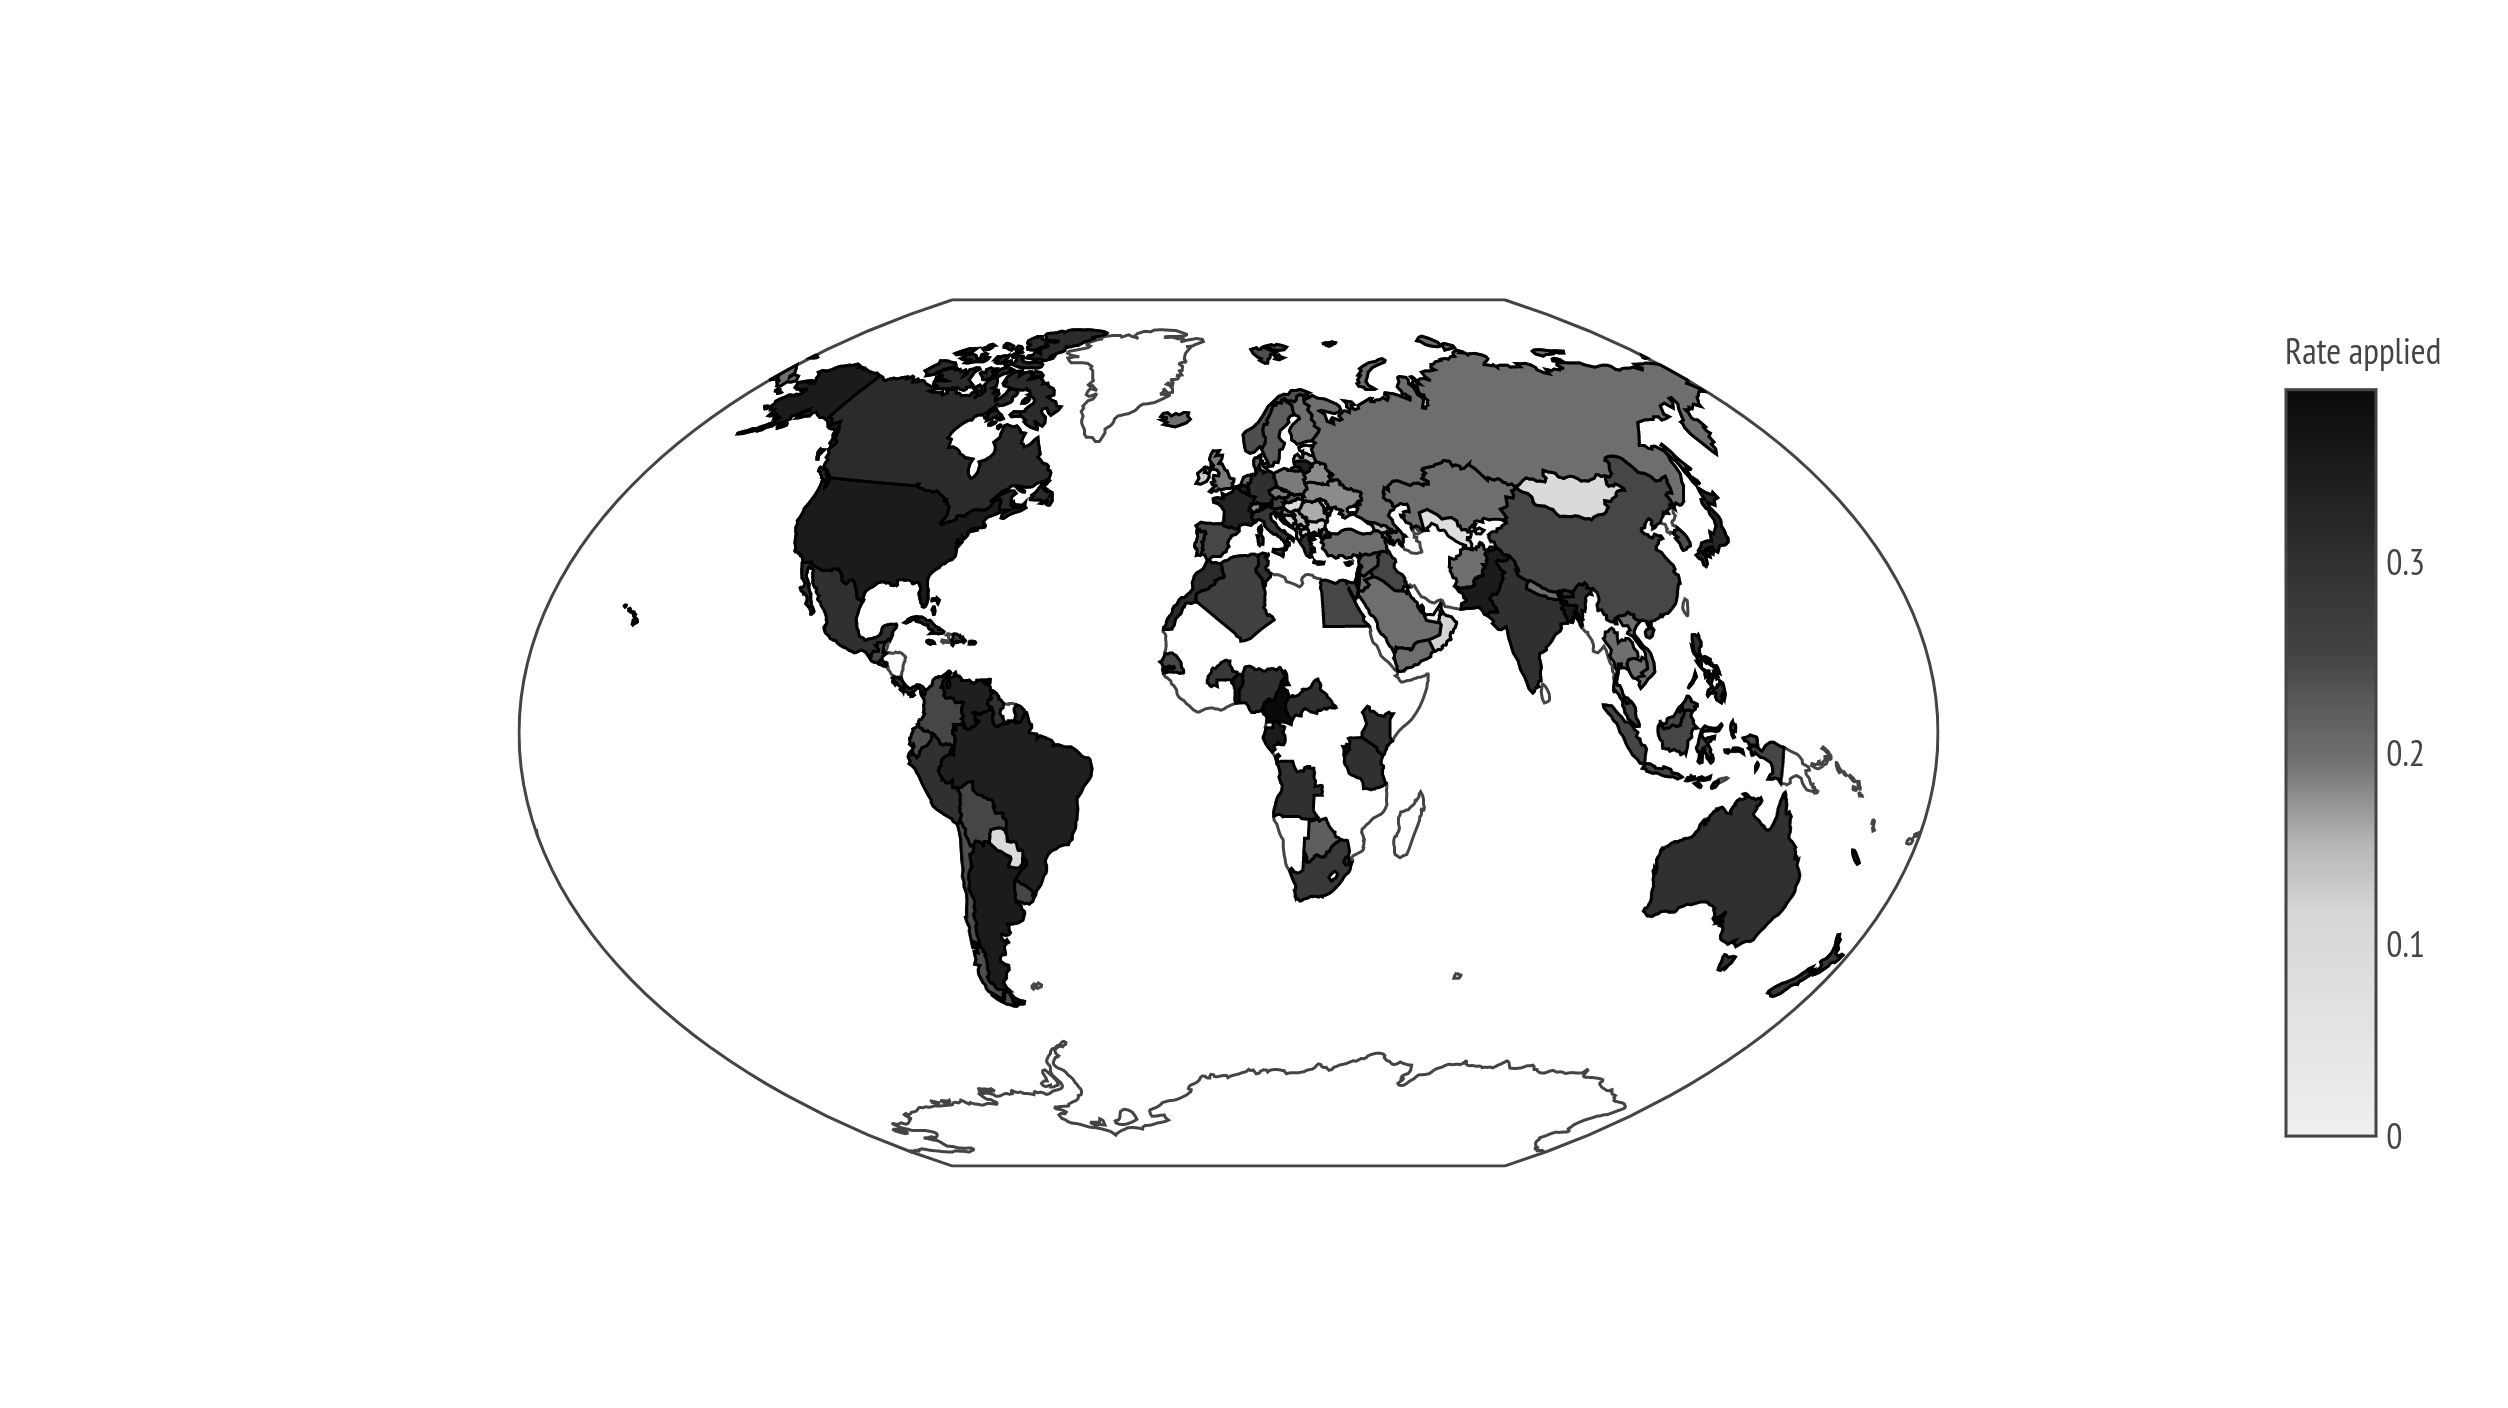
\includegraphics[width=1\linewidth]{Images/CTworld.png}
  \caption{Corporate Tax around the world}
  \label{fig:test1}
\end{minipage}%
\begin{minipage}{.5\textwidth}
  \centering
  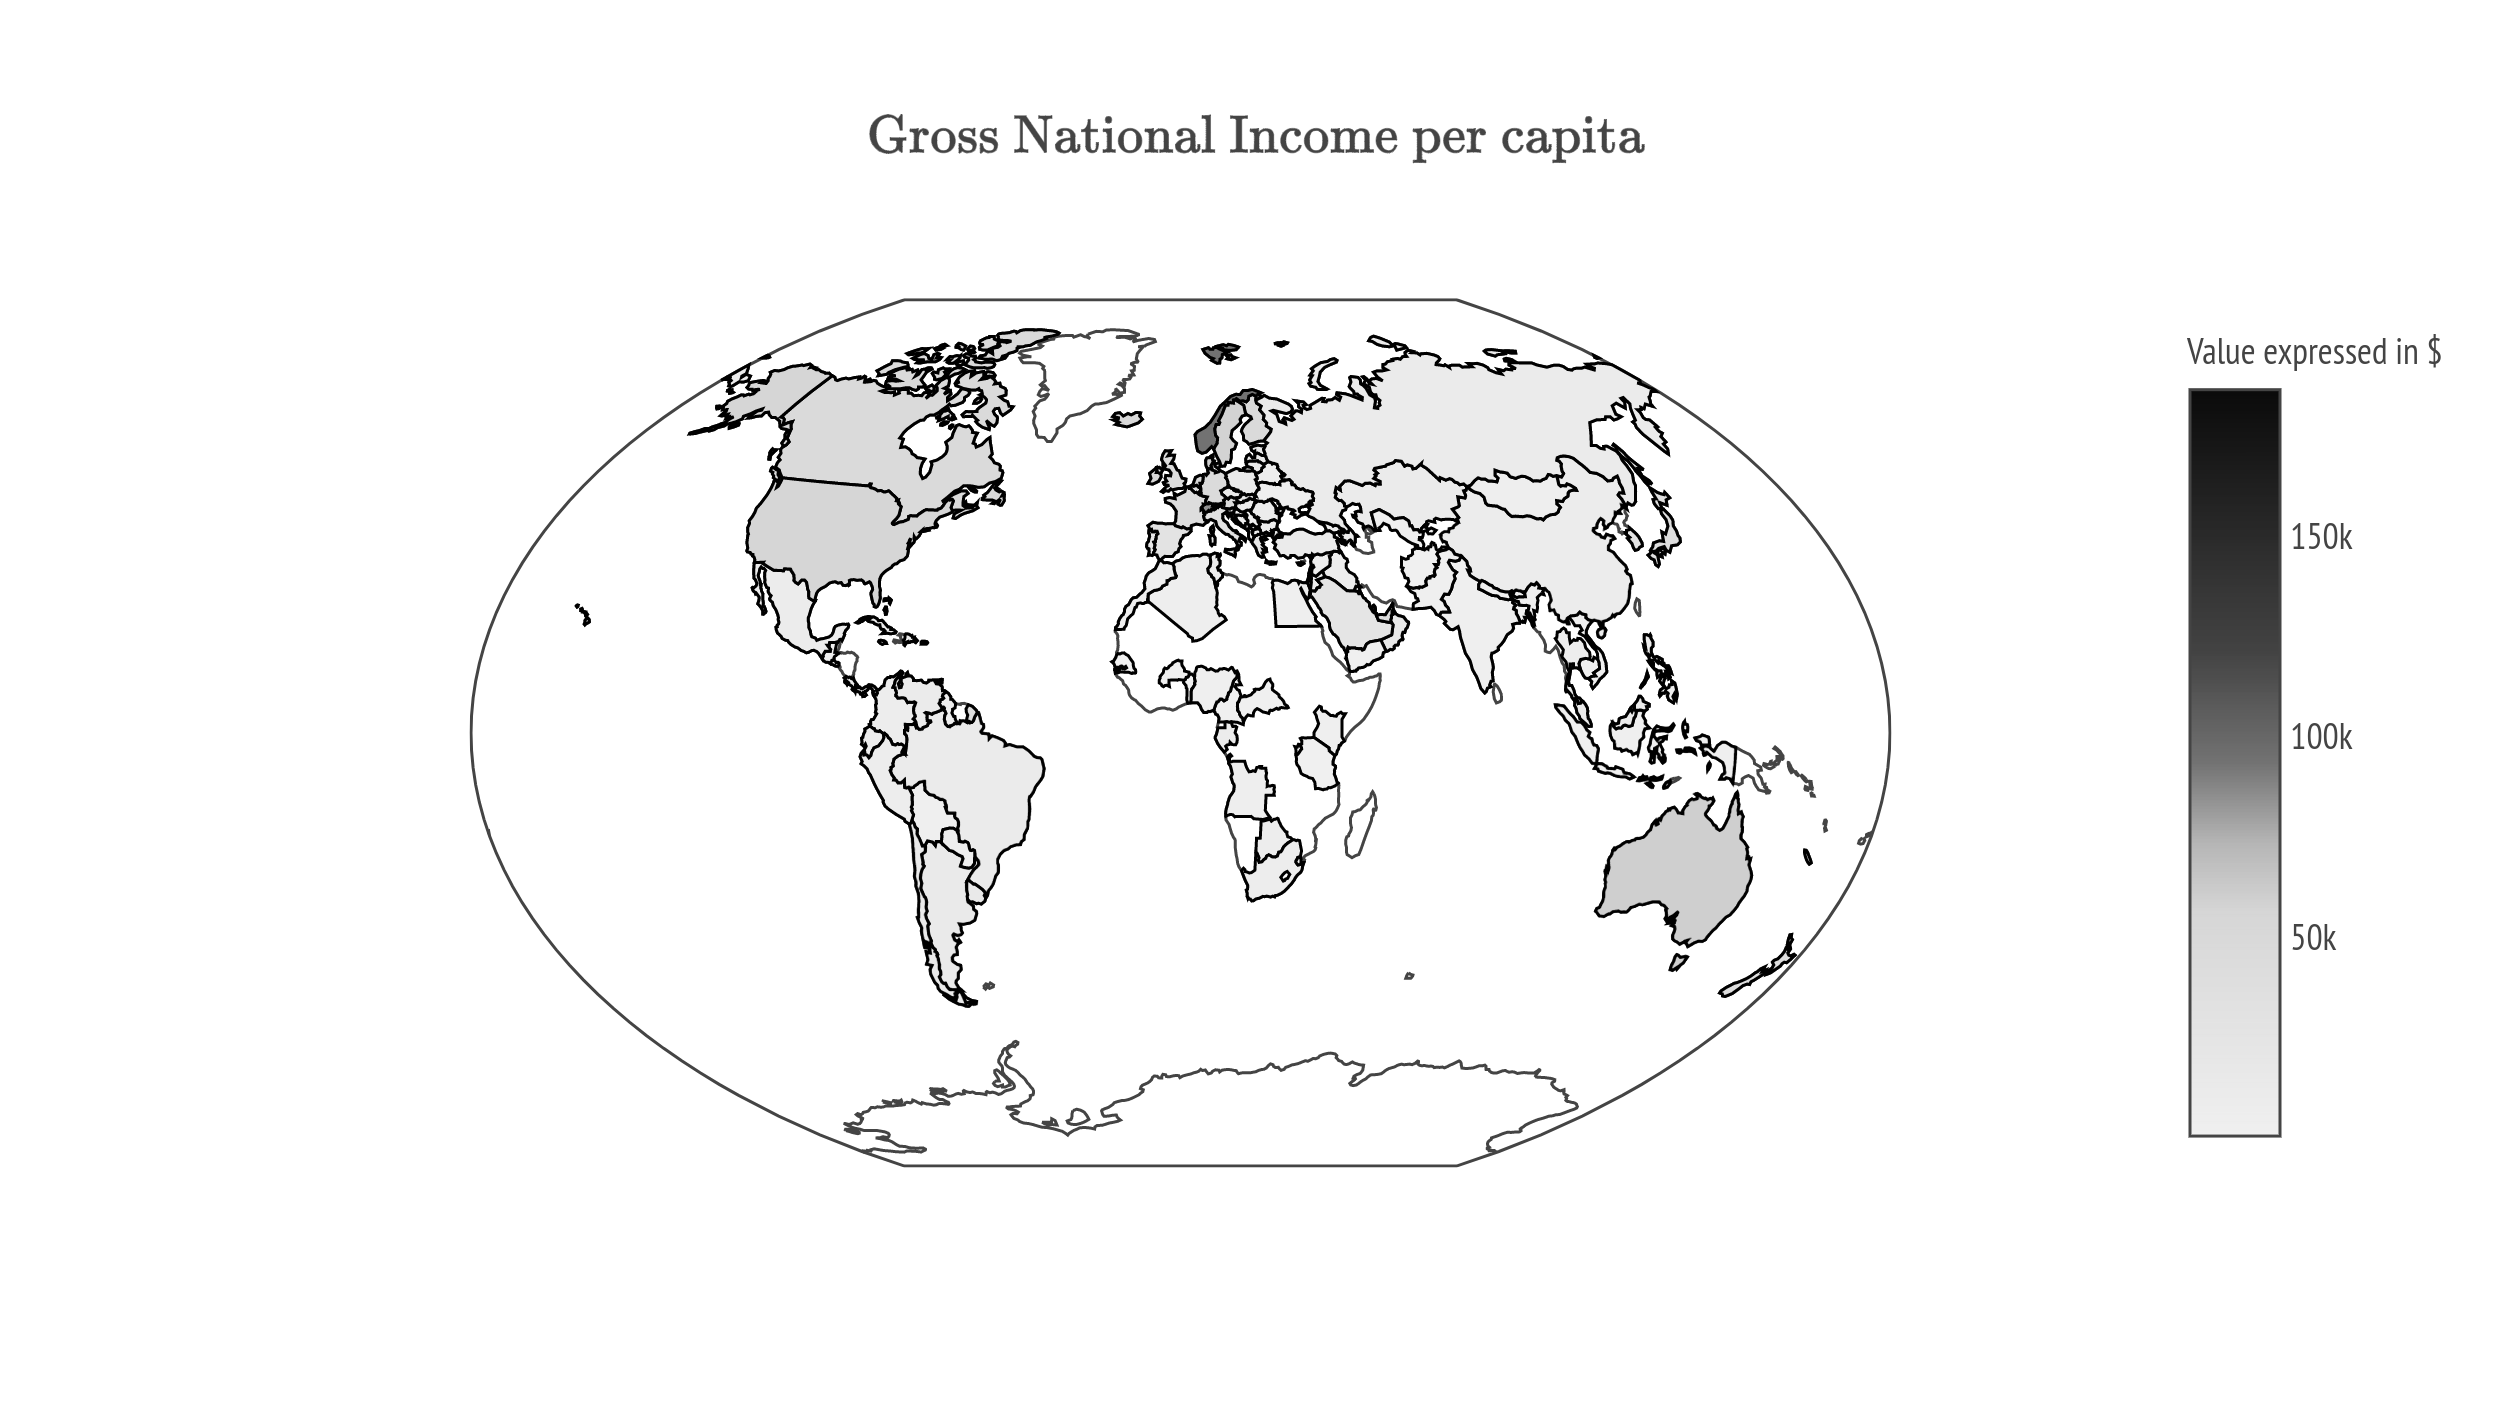
\includegraphics[width=1\linewidth]{Images/GNIworld.png}
  \caption{Gross National Income per capita}
  \label{fig:test2}
\end{minipage}
\end{figure}

\begin{figure}[ht]
\centering
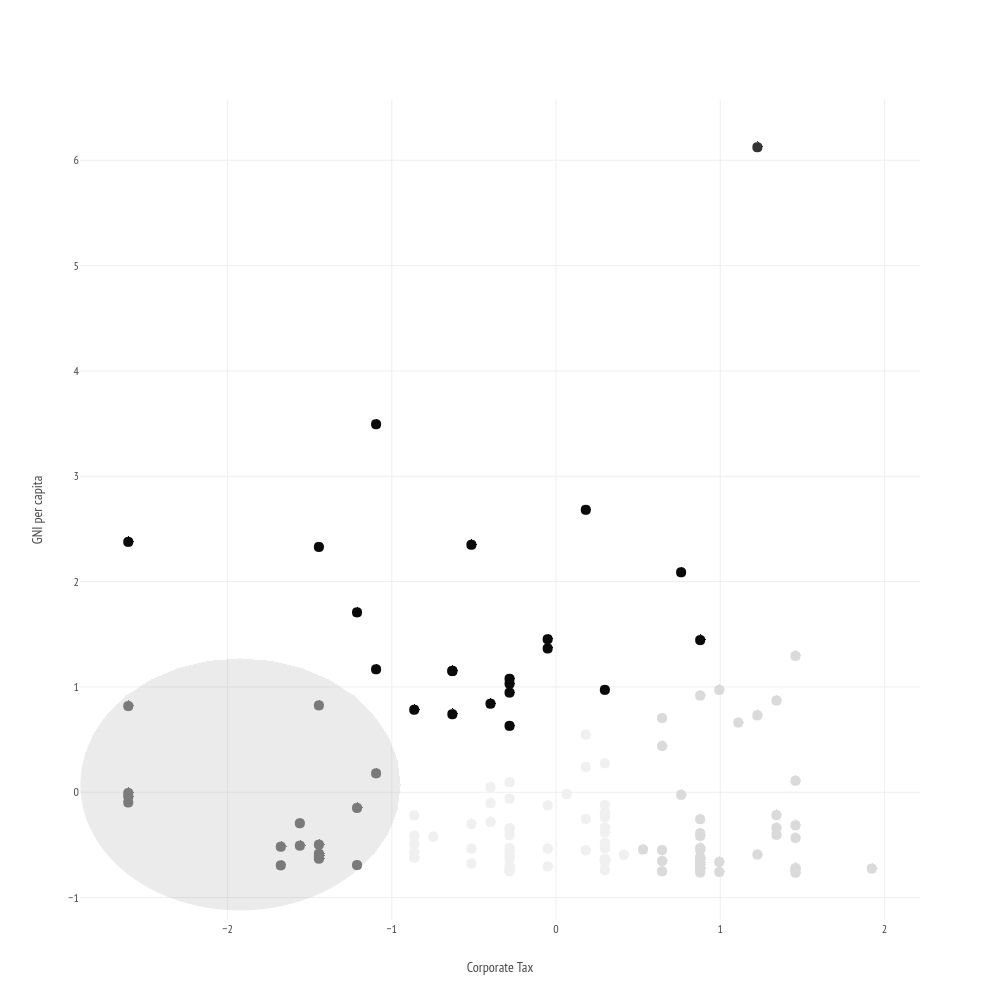
\includegraphics[width=0.8\linewidth]{Images/Cluster-GNI-CT.png}
\caption{K-mean cluster on standardized Corporate Tax and GNI per capita}
\end{figure}

Figure 4 shows a scatter plot of the normalized Corporate Tax (x axis) and GNI per capita (y axis), to such data I applied a K-mean cluster algorithm with K=5, this kind of algorithm randomly assigns each observation to a cluster, and finds the centroid of each cluster then, through iteration reassign data points to the cluster whose centroid is closest and calculate the new centroid of each cluster. The K was chosen with the "elbow method" with $R^2$ meaning that 5 was the number of cluster that return the best trade off in terms of $R^2$ increase and and cluster numerosity.
The result were five clusters with the one highlighted by the circle indicating countries with both a low average cost of worker and a low taxation. However even if these may seem the best locations to allocate the entities this is not always true, since the formula for taxation is the one proposed at section 4.2 and such entities have to be in the range proposed in section 4.3.

\subsubsection{Target enterprise data}

This data includes the information we got from our enterprise (the one in which we're going to reallocate the entities). Even though, the data that can be extracted from the enterprise are enourmous, the decision was to depict the most valuable information on the enterprise keeping under controll the numerosity of such parameters. The parameter identified are: 
\begin{itemize}
	\item Revenues: they represent the upper limit in which, whether crossed, our strategy will result not profitable, this element can be either forecasted or in case of a constant flow of revenues over the years we can use historical data;
	\item Employees: this element is somehow tied to the revenues we expect to have, plus some limitations dictated by the labour unions depending by the countries (which were not modeled);
	\item Cost of running the asset: this is a very crucial factor in case of business that rely heavily on machinery and industrial plant activities, in fact such parameter may be neglected or, take a secondary position in the decision process, in case of a business relying heavily on employees, as for example a software company or a consulting firm.
\end{itemize}

While obtaining the first two parameters is something not particularly intensive in terms of data gathering and may require some additional effort the forcasting part because of the uncertainty that some industries carry. In case of the cost of running the assets we have two choices, we can either use internal data coming from a unified ERP system or use the single entity financial data and try to forecast each single entity cost of running the asset and then scale it to a common base in order to do an "apple to apple" comparison. In order to extract such parameter we can use the operating expenses of the entity\cite{williams_financial_2008}, subtracting from the operating expenses the wages we can obtain the information inherent the cost of running the assets at a certain time $t_0$ for a certain volume of good $V_0$, dividing the cost of running the asset for $V_0$ will give a proxy of the marginal cost of asset given an increase of the production by one unit. This procedure has to be intended as measure of last resort in case of a non unified ERP system which still is the most reliable source of data in case of global entities located in very different countries. 
\\
\\
It's worth noting that are part of the enterprise data other information which are not part of the above mentioned parameters, such data deals with the DM preferences andsome of them may involve limits in the numerosity of the number of entities. In some cases a large number of enterprise can result in a trade off between potential synergies and the cost of keeping a costant flow of goods and information to them. This prefecernce can narrow down till the functional characterization of an entity and may involve the localization in a particular country because of the public image of the Group.

\subsubsection{Global enterprises data}
This category contains all the data inherent the PLI of the specific functional enterprises operating in a certain State.
A piece of this data is summarized by the following representation. Another important data that can be obtained is the cost of debt \cite{berman_financial_2013} even though such measure has to take into account the proportion of two types of funding (namely equity and debt) the data provided by the comparable enterprises serve as a good proxy for such measure if used in conjunction with financial databases as Bloomberg. In our case, to obtain this data a private worldwide database was used called Orbis by Bureau Van Dijk.
\begin{sidewaysfigure}
\centering
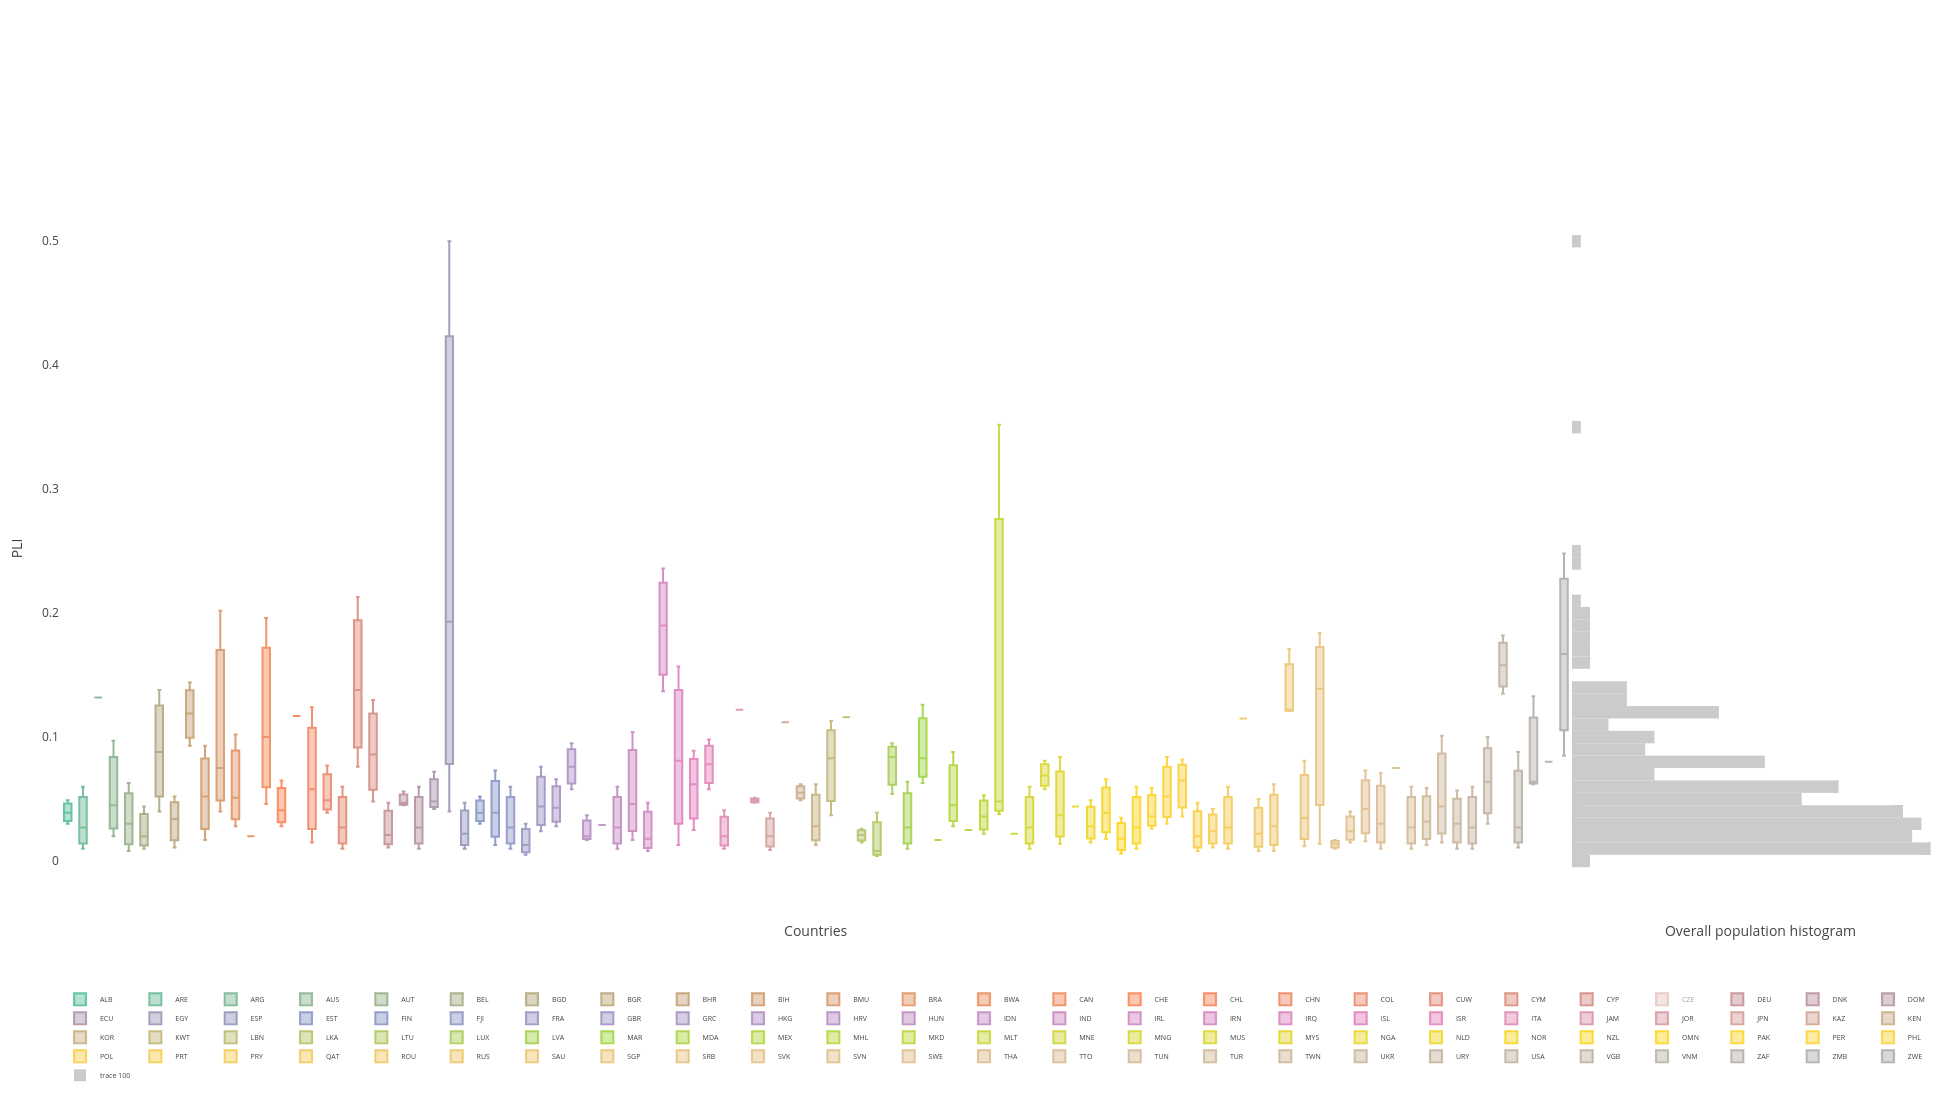
\includegraphics[width=\textwidth]{Images/plidist.png}
\caption{Interquartile range of distribution PLI sorted by country}
\label{fig:interquartile}
\end{sidewaysfigure}

In the figure \ref{fig:interquartile}, we can see how the PLI interquartile range changes from country to country in such case the PLI we choose was an ROS applied on independent companies whose activities are based on distribution (from wholesale to retail). Such difference can play a major role in deciding the optimal profitability level of the allocated entities. The PLI, acronym of Profit Level Indicator is the a financial indicator (most of the time a ratio) that tracks the profitability of a certain function performed by the entity under scope of analysis.

\subsection{Objectives}
The data reported above will be used to set up the GP model and constitutes part of the objectives and constraints that will be presented below. In order to model the overall allocation we need to take into consideration the following:
\begin{itemize}
    \item The overall cost of production should be minimized;
    \item The tax liability should be minimized;
    \item The profit should be divided among the entities based on the contribution that such entity give to the overall process of value creation;
    \item The functional characterization of each entity must fall within a range achieved by comparable non controlled entities.
\end{itemize}

\subsubsection{Cost minimization}
This is a very basic objective in which we try to minimize the cost embodied in each national entity. The cost function for each entity is primarily given by three variables, namely employees (which constitute the major variable cost of an enterprise) then we have the specific cost of running the assets (machinery, offices etc...) and then we have the cost of capital (meaning the remuneration expected share holders and financiers). All these variables contribute to the determination of costs. The approximation function derived will look as follows:

\[
C(E,A,K)=ce_k\cdot E+ca_k\cdot A+ck_k\cdot K \quad \forall k \in \left\{1...N\right\}
\]

Where (1)$ce_n$ corresponds to the National Income per Capita, this index was chosen because of its availability through the nations at scope and because it's a good proxy for the cost of labour in each State; (2)$ca_n$ corresponds to the cost of running the assets and is derived as illustrate before by subtracting the wage cost to the operational expenses and then adjusting for the purchasing power; (3)$ck_n$ corresponds to the cost of capital (in our case debt) calculated using data from comparable companies.
Even if this three variables do not represent the full cost structure of each enterprise (cost of good sold was not mentioned) is helpful for the decision maker to take into account this three driver of cost since this information constitutes the main driver to address value adding activities in the overall value chain.

\subsubsection{Tax base minimization}
This objective is the crucial point of this work since an optimal tax strategy can be considered good for profit maximization. However, should be mentioned that this doesn't constitute any avoidance of taxes but a strategy to be competitive in the market. Such allocation result as the consolidate minimization of all the national tax base, which is given by subtracting from the revenues allocated to a particular State ($y_k \cdot R$) the cost allocated to the same State (here expressed as $x_k \cdot C(E, A,K)$. This residual forms the EBIT (namely Earnings Before Interest and Taxes), by multiplying this the EBIT by the national corporate tax we get the Tax Base. The tax base function will look as follows:

\[
T(R,E,A,K)= [R-(ce_k\cdot E+ca_k\cdot A+ck_k\cdot K)]\cdot tx_k \quad \forall k \in \left\{1...N\right\}
\]

\subsubsection{Functional allocation}
This objective derives from the TNMM technique used in accessing the transfer pricing goodness. The method is based on the examination of the net profit relative to an appropriate base (e.g. costs, sales, assets) that a local entity realizes from a controlled transaction (or in our case to the entity itself). Basically, we introduced this objective as a quality control that the overall process of maximization of profits as some confirmation also in the real market, made by independent actors. This is in certain sense a bond that helps the model in giving a solution viable also in an anti avoidance perspective.

In order to do so we first need to identify which Profit Level Indicator to choose; this is an important choice that has to be made taking into account the functional characterization of such entity, that is, if an entity focuses on distribution the best PLI to test such entity is given by the ROS of its functional characteristics, that's because the sales are supposed to be the main element of a distributor (and not cost or assets). The main PLI used by practitioner are: Return on Sales, Full Cost Mark-up, Return on Asset, Return on Investment.

After we matched each functional characteristic with its relative PLI we need to find the data of comparable independent entities, in order to asses the profitability range that our entity has to obtain to be in an arm's length position.

The objective function returning such objective would be as follows:

\[
\begin{cases}
   \frac{R - C(E,A,K)}{R} & \text{if } q=1
   \\
   \frac{R - C(E,A,K)}{C(E,A,K)} & \text{if } q=2
   \\
   \frac{R - C(E,A,K)}{A} & \text{if } q=3
   \\
   \frac{R - C(E,A,K)}{E} & \text{if } q=4
\end{cases}
\]
The basic idea behind this objective is that for a moment we're forgetting about the group objective (the first and the second) that try to minimize the consolidated cost and tax base. In this case we're focusing on the profitability of each entity.

\subsection{Profit split}
This objective is represented by the goals (4)(5)(6) and the methodology used to determine this type of split derives from the profit split method used in transfer pricing analysis. In particular the transfer pricing profit split aims at: determining the division of profits that independent enterprises would have expected to realize from engaging in the transaction \cite{OECD_ProfitSplit_2017}. In our case we'll use this method and particularly the contribution analysis to define the effort of each functional category in the value chain. Secondly we'll use this value driver to partition the profits in order to have, at the en, a structure that takes into account the internal value chain of the products and not just the information gained by independent comparable companies.


\subsection{Constraints}
Constraints represent the boundaries where the system will result unfeasible. Such constraints are expressed by the equation from (7) to (15); where the first two represent the boundaries on the PLI distribution namely the lower quartile and the upper quartile, outside this range the profitability may not be considered to be arm's length. The constraints (10)(11)(12)(13) represent the frontier of the possible allocable resources given by the company under the scope. The constraints (13),(14) and (15) sets the positiveness of the deviation variables in order to avoid incorrectness of the overall GP model.

\subsection{Goal Programming Model}

This model aims to find the best allocation of costs and budgeted revenue in order to maximize profits minimizing costs and tax base, at the same time the model provides the best multinational functional allocation strategy to achieve such goal using both internal and external data from independent companies.
The objectives are divided into two categories; the first one is given by three objectives namely cost minimization, tax base minimization, PLI coherence; the second focuses more on the control and limitations that the decision maker wants to implement in the model due to the specific characteristics of its business.

The overall model algebraically looks as follows:

\[ \min_{p,n} \quad \sum_{i=1}^{Q} (\prescript{}{q}{p}_i \cdot w_i) + w_3 \cdot \sum_{i=1}^{O} (\prescript{}{o}{n}_i) + w_4 \cdot \sum_{i=1}^{N} ( \prescript{}{n}{n}_i + \prescript{}{n}{p}_i )\]


\begin{numcases}{Subject \quad to}
   \sum_{q=1}^{N} C_q(E,A,K) - \prescript{}{q}{p}_1 = 0
   \\
   \sum_{q=1}^{N} T_q(R,E,A,K) - \prescript{}{q}{p}_2 = 0
   \\
   P_k(R,E,A,K)+\prescript{}{n}{n}_k-\prescript{}{n}{p}_k =V_k  \qquad \forall k \in \left\{1...N\right\}
   \\
    \sum_{q=1}^{D} (R_q-C_q(E,A,K))+\prescript{}{o}{n}_1 = c_1\cdot \sum_{q=1}^{N} (R_q-C_q(E,A,K))
   \\
    \sum_{q=1}^{P} (R_q-C_q(E,A,K))+\prescript{}{o}{n}_2 = c_2\cdot \sum_{q=1}^{N} (R_q-C_q(E,A,K))
   \\
    \sum_{q=1}^{M} (R_q-C_q(E,A,K))+\prescript{}{o}{n}_3 = c_3\cdot \sum_{i=q}^{N} (R_q-C_q(E,A,K))
   \\
   P_k(R,E,A,K) \geq L_k  \qquad \forall k \in \left\{1...N\right\}
   \\
   P_k(R,E,A,K) \leq U_k \qquad \forall k \in \left\{1...N\right\}
   \\
   \sum_{q=1}^{N} R_q = R^*
   \\
   \sum_{q=1}^{N} E_q = E^*
   \\
   \sum_{q=1}^{N} A_q = A^*
   \\
   \sum_{q=1}^{N} K_q = K^*
   \\
   \prescript{}{q}{p}_i,\prescript{}{q}{n}_i \geq 0 \qquad i=1,...,Q
   \\
   \prescript{}{n}{p}_i,\prescript{}{n}{n}_i \geq 0 \qquad i=1,...,N
   \\
   \prescript{}{o}{p}_i,\prescript{}{o}{n}_i \geq 0 \qquad i=1,...,O
 \end{numcases}


As you can see the (1)(2)(3) belong to the first category, where instead (4)(5)(6) belong to the second, the latter in fact depend on the strategy of the decision maker and it's not given by any environmental variable.

\pagebreak

\section{Mathematical simulation: a case study}
The simulation of the above-mentioned model was made using LINGO17. Even if the mathematical package was able to handle the total amount of data given by the model the simulation was done using a portion of this data, avoiding countries in which the company doesn't operate at all. Other limitations were implemented in order to avoid any possible nonlinearity, resulting in an increase of the computational time to obtain a solution, this was possible by avoiding inserting the equation (3), when instead the correlated constraints, namely (7) and (8) were linearized. Other limitations to the model are exposed below:
\begin{itemize}
    \item The PLI chosen to set the functional range were only 2, ROS and FCMU;
    \item The cost of asset and equity was set to 0, meaning that the only cost driver was employees;
    \item The functional characterization was reduced to 3, namely distributor, producer and principal (which acts as an active holding);
    \item The number of employees was assumed to be continuous, meaning that part-time work and non full year worker can be used by the firm.
\end{itemize}

Concerning the data, the financial were taken from a company operating mostly in Europe and western countries in general, plus this company tend to produce and store most of its products in Asian countries and tend to have less inventory in its western distribution sites. The company under scope was under performing at the time of this simulation its P/L statement registered a loss of roughly  6.960.502 USD. The revenues registered for the year under the scope were about 88.900.344,00 USD and the employees hired were 2.722,00.
The weights were chosen in order to value firstly the tax minimization, then the contribution of each entity on the profit made by the company (profit split) and the cost minimization.

\subsection{Conclusions}
The results produced by the mathematical package are illustrated in the following table:

\begin{center}
 \begin{tabular}{||c c c c||}
 \hline
 State & Function & Revenues allocation & Employees allocation \\ [0.5ex]
 \hline\hline
 Cyprus & Distributor & 7.986.031 & 269,2824 \\
 \hline
 Denmark & Manufacturer & 5.464.000 & 57,5619 \\
 \hline
 Latvia & Principal & 64.144.930 & 2.295,3010 \\
 \hline
 Portugal & Principal & 11.305.390 & 99,8544 \\
 \hline
\end{tabular}
\end{center}

The financial data of the company shown an average consolidated tax burden of 21\% where instead using the model we achieved a rate of 17\% the only periods where such a ratio where lesser than the one achieved by the model where the one in which the company started to register losses (that caused a decrease in the tax burden). This model, fixing the PLI at a positive level doesn't allow any combination to result in an EBIT of 0 consequently the only achievable 0 rate may be in case of a tax haven.

The deviation variables we used registered the following discrepancies:

\begin{center}
\begin{tabular}{|| L  L L ||}
\hline
\text{Variable} & \text{Amount} & \text{Description} \\
\hline
\prescript{}{q}{p}_1 & 46.870.020,00 & \text{Consolidated cost of employees} \\
\hline
\prescript{}{q}{p}_2 & 7.159.194,00 & \text{Consolidated tax liability} \\
\hline
\prescript{}{o}{n}_1 & 0,00 & \text{Distributor profit allocation} \\
\hline
\prescript{}{o}{n}_2 & 0,00 & \text{Manufacturer profit allocation} \\
\hline
\prescript{}{o}{n}_3 & 0,00 & \text{Principal profit allocation} \\
\hline
\end{tabular}
\end{center}

The model is far from being used as the only tool that decision makers can use to solve problems of business restructuring, however, the result shows that multi criteria analysis and especially goal programming may constitutes one of the best tools that can be used to measure such decision.


\newpage
\emergencystretch=1em
\sloppy
\printbibliography
\end{document}

	%===========================
	\documentclass{article}

\usepackage{amsmath}
\usepackage{mathtools}
\usepackage{amstext}
\usepackage{array}
\usepackage[backend=biber,
            url=false]{biblatex}
\usepackage{float}
\usepackage{tikz}
\usepackage{txfonts}
\usepackage[colorinlistoftodos]{todonotes}
\usepackage[long]{optidef}

  \addbibresource{ch1-2.bib}

  \usetikzlibrary{calc,matrix,decorations.markings,decorations.pathreplacing}
  \usetikzlibrary{positioning}

  \definecolor{colone}{gray}{0.7}
  \definecolor{coltwo}{gray}{0.6}
  \definecolor{colthree}{gray}{0.5}
  \definecolor{colfour}{gray}{0.9}
  \definecolor{colfive}{gray}{0.9}
  \definecolor{colsix}{gray}{0.9}
  \definecolor{colseven}{gray}{0.9}

  \tikzset{
  table/.style={
  matrix of nodes,
  row sep=-\pgflinewidth,
  column sep=-\pgflinewidth,
  nodes={rectangle,text width=2cm,align=center},
  text depth=1.25ex,
  text height=2.5ex,
  nodes in empty cells}
  }

  \tikzstyle{startstop} = [rectangle, minimum width=2cm, minimum height=1.5cm,text centered, draw=black]
  \tikzstyle{process} = [rectangle, minimum width=3cm, minimum height=1.5cm, text centered, draw=black]
  \tikzstyle{blank} = [circle, minimum width=0.1cm, minimum height=0.1cm, text centered, draw=white]
  \tikzstyle{arrow} = [thick,->,>=stealth]

\begin{document}

  \title{Chapter 2}

  \author{M. Repetto}

  \date{}

\maketitle

\begin{abstract}
  In the following paper is proposed a multi-objective model for components allocation in a Green Supply Chain framework. The model builds on the concept of the supply chain as suggested by Porter, and accounts for the costs of production using the Activity Based Cost accounting method (ABC). Such model is organized in blocks related to several moments in the value chain, from the procurement to the end customer. Above each and every one of these blocks, we included a series of environmental constraints that the firm has to comply, with respect to specific country regulation, or in case of a particular Corporate Environmental Responsibility policy...\todo{Da continuare quando il modello è ultimato; inserire anche parte sui risultati}
\end{abstract}

\section{Introduction}
  Global Supply Chain Management (GSCM) is probably one of the most used terms when we talk about how the firms are running their business nowadays. GSCM may be defined as the allocation of goods and services along a series of transnational companies' global network to maximize profits and minimize waste. As the Supply Chain Professionals puts it, the goal of GSCM is threefold and focuses on delivering: (a) the right product (b) to the right place (c) at the right time.
  Inside this very wide paradigm, we can find the concept of logistics which is in charge of the movement of goods, service and last but not least information from the sourcing of raw material, till it reaches the end customer.
  Along with these two concepts a third one stucks with them, the Green Supply Chain (GSC). This idea, brought to light by a more advanced concern about environmental matters of the developed countries, forced the firms to be accountable for their negative externalities related to the environment in which they operate \cite{srivastava_green_2007}.

  However such legislation lacks from a point of view of legal constraints, setting only a few qualitative restriction, poorly measurable by the enterprises or in some cases letting the customers pay for their environmental behavior toward waste disposition. These facts are inevitably leaving some degrees of freedom to the firms, on the other hand, is also important to notice that these are only seeds of legislation that show us how the long-term trend will be about the tolerance given to the behavior of firms with environmental concerns, a trend that in the future may require firms to set particular frameworks to be accountable for their environmental impact. Nowadays such effort is not achieved by the legal frameworks provided by the domestic legislators but by the Corporate Environmental Responsibility (CER), meaning that are the stakeholders to impose the companies to be more responsible on their day to day operations.

  Looking at the literature, we can see that there is an emerging branch which deals with the Green Supply Chain Management, a new paradigm of Supply Chain Management whose aim is to keep under control the behavior of the firm during its operations, by applying policies such as Green Manufacturing and Remanufacturing, Green Design etc...

  Because of that we propose a Goal Programming model in order to address such problems, following what proposed by literature we try to enhance such model fixing quantitative and qualitative constraints to the pollution generated by the value adding activities, involved in the creation of the good and we also try to implement the benefits of a recycling program enacted by the firm apropos the WEEE directive.

  In our case, we chose the networking electronic appliance business (i.e. hub, switch or router).\todo{Il business può cambiare ad oggi ho trovato pochissimi dati a riguardo non avendo più accesso ai database aziendali}  In order to measure such impact, we'll use the framework provided by the Activity Based Costing, in order to assess and address the marginal environmental impact of any additional unit elaborated by the transnational firms.

\section{Green Supply Chain}
  Green Supply Chain may be defined as the series of interconnected activities across the border of different enterprises that adds value to the goods and services from the sourcing to the market. Its aim is to improve performance in measures of sustainability, cost reduction, emission reduction. Whereas Supply Chain Management sets its objectives to maximize profits and minimize waste, in economic terms, Green Supply Chain sets its objectives even further, posing as its ultimate mission to lower the ecological impact that a firm or a series of them has in their day to day operations. Such operations may involve:
  \begin{itemize}
    \item Green Manufacturing and Remanufactoring: is the process of controlling and reutilizing material in the manufacturing, in order to limit waste creation\cite{urvashi_green_2013};
    \item Green Design: is an approach put in place to promote the environmental quality of a certain product or service,  by reducing negative impacts on the natural environment; an example could be the automatic switch of the television after a period of idleness\cite{ceschin_evolution_2016}; and
    \item Green Operations in general: by green operation we mean any type of activity which does not fall into the two categories mentioned above but is characterized by a "green" attitude as for example the optimization of the offices consumption through a remote-working policy;
  \end{itemize}

  In the market under scope which is the European one, there are several legislation concerning the environmental impact of certain eProducts\footnote{for eProducts, we intend electrical and electronic equipment such as computers, TV-sets, fridges, cell phones and other electronic appliances}. The most important are:
  \begin{itemize}
    \item Waste Electrical \& Electronic Equipment (WEEE);
    \item Restriction on Hazardous Substances (RoHS): ;and
    \item Ecodesign Requirement for Energy-using Product (EuP): :
  \end{itemize}

  Such legal frameworks act at different levels from the sourcing to the customer involving community member States. The following flowchart illustrates this differences.

  \begin{figure}
    \centering

    \begin{tikzpicture}[scale=0.8, every node/.style={scale=0.6}]
    \node (start) [startstop] {Design};
    \node (process1) [process, right=of start] {Production};
    \node (process2) [process, right=of process1] {Distribution};
    \node (process3) [process, right=of process2] {Use};
    \node (process4) [process, right=of process3] {Disposal};

    \draw [arrow] (start)--(process1);
    \draw [arrow] (process1)--(process2);
    \draw [arrow] (process2)--(process3);
    \draw [arrow] (process3)--(process4);

    \draw[decorate,decoration={brace,mirror,raise=10pt}]
    (start.south west) -- (start.south east) node[below, midway, yshift = -20]  {EuP};
    \draw[decorate,decoration={brace,mirror,raise=25pt}]
    (start.south west) -- (process1.south east) node[below, midway, yshift = -45]  {RoHS};
    \draw[decorate,decoration={brace,mirror,raise=45pt}]
    (process1.south west) -- (process4.south east) node[below, midway, yshift = -80]  {WEEE};

    \end{tikzpicture}
    \caption{Legislation affection}
  \end{figure}

  In the following subsection, an additional overview is given to such legislation.

\subsection{Waste Electrical \& Electronic Equipment}
  The Waste Electrical \& Electronic Equipment also called WEEE is ruled in the European Community by Directive 2002/96/EC now repealed by the Directive 2012/19/EU \todo{Non ho citato esplicitamente la direttiva nelle fonti, nei paper che ho letto nessuno tende a farlo, nel caso fosse necessario provvederò a farlo}. The objectives of the policy are, to preserve, protect and improve the quality of the environment, to protect human health and to utilize natural resources prudently and rationally. That policy is based on the precautionary principle meaning that the polluter should pay for its damage. Is important to notice that in the European market such directive is impacting all the community members is not perfectly homogeneous ways because of the implementation which is remitted to the local authorities. This problem may incur in potential elusive behavior as highlighted by the German firms who exploited gaps in the law which have allowed them to move large amounts of WEEE declared for recycling to developing economies including India, China, Nigeria and Eastern Europe \cite{ongondo_how_2011}. Despite such cases, the overall impact of this directive is mostly positive as highlighted by the Eurostat data here exposed.

  The WEEE Directive currently sets a minimum collection target of 4 kg per year per inhabitant for WEEE from households. From 2016, the minimum collection rate shall be 45\% calculated on the basis of the total weight of WEEE collected. Where the WEEE is calculated with the following formula:
  $$
  W (n) = \sum{t = t_0}_{n} POM \cdot L^p(t,n)
  $$
  Where $W(n)$ refers to the specific quantity of electrical and electronic waste for a specific year, $POM(n)$ is the quantity of new electrical component injected in the market and $L$ is the discard-based lifespan profile for the electrical component injected in the market. From the graph proposed below we can see how the target of minimum collection of 4 kg per year per inhabitant for WEEE from households was achieved by all the countries in the Eurozone however not all the countries has the same collection rate, meaning that some of them may have introduced legislation that comply only with the minimum target of the directive, leaving the households with the freedom to dispose of their WEEE in unconventional manner. Clearly this means for the enterprises less obbligation on the collection of eProducts, but at the same time less products to be recicled and less opportunity of remanufactuirng.

  \begin{figure}
  \centering
  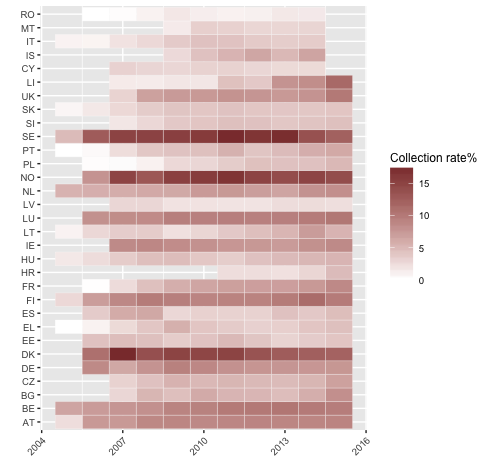
\includegraphics[width=0.8\linewidth]{Images/heatmap.png}
  \caption{Kilograms of WEEE collected per capita}
  \end{figure}

\subsection{Restriction on Hazardous Substances}
  The Restriction on Hazardous Substances also called RoHS is represented by the Directive 2017/2102 (RoHS 2 recast). The scope is the restriction on the use of certain hazardous substances in electrical and electronic equipment (EEE) such as lead, mercury, cadmium, hexavalent chromium etc... In such case, as opposed to the WEEE the RoHS directive acts as a barrier to the products containing such minerals and not when they become waste. In considering such regulation is worth noting that there are no differences between the dimension of the distributing entity, meaning that small businesses, as well as large businesses, are equally affected by these restrictions. The only amendment is given to the batteries that may exceed such restriction.

\subsection{Ecodesign Requirements for Energy-using Product}
  The Directive 2009/125/EC is meant to deal with Ecodesign regulations, ecodesign regulations require manufacturers to decrease the energy consumption of their products by establishing minimum energy efficiency standards. In particular, The Ecodesign Directive provides a consistent legal framework for improving the environmental performance of products setting out a minimum mandatory requirement for the energy efficiency of theseProducts. In case of the design of IT networking products such as routers and switches the firms are obliged by such directive to implement some ecodesign features such as the maximum wattage of 1W in case of off mode or a standby maximum consumption of 2W. Such measure per se do not impact in any case the supply chain since they are just additional features that has to be implemented in theProducts sold in Europe.

\section{A state of the art review \todo{Per ora ho riposrtato solo i paper che ho letto, man mano che li leggo li aggiungo}}
  As proposed by the Council of Supply Chain Management Professionals, the Supply Chain Management (SCM) is the planning and the management of all activities involved in sourcing and procurement, conversion, and logistics as well as coordination and collaboration with the entities. The problem arising from such activities seems to be well addressed by mathematical modeling, other advantages of such approach are the economic sustainability and the possibility to scale the model in order to address different situations.
  From the comprehensive review built by Muna et al. \cite{mula_mathematical_2010} we discovered the methods used by the academic world and the specific situations the tried to model, which are:
  \begin{itemize}
	  \item Linear Programming: order quantinty definition by means of decentralization\cite{jung_order_2008}, production and distribution planning taking into account country specific regulations\cite{Oh_Karimi_2006}, multiple points of sales planning\cite{Kanyalkar_2005};
	  \item Mixed Integer Linear Programming: network optimization and routing configuration\cite{romo_optimizing_2009}, distribution planning in an environment with just a production plant and many distribution centers\cite{Rizk_Martel2008};
    \item Non Linear Programming: optimization of production, transport and inventories\cite{benjamin_analysis_1989};
    \item Multi Objective Programming: replenishment production and distribution planning with conflicting objectives simultaneously\cite{torabi_interactive_2008}, master planning\cite{Chern_Hsieh_2007};
    \item Fuzzy Mathematical Programming: distribution allocation considering different products and production/distribution centers\cite{Liang_Cheng_2009};
    \item Stochastic Programming: addressing demand uncertainty accounting for the probability distribution\cite{Gupta_Maranas_2003};
    \item Heuristics Algorithms and Meta-Heuristics; and
    \item Hybrid Models.
  \end{itemize}

  Is worth noting how the majority of the models pertain to the category of Mixed Integer Linear Programming, this may be due to the fact that is probably one of the simplest and most reliable methods that can be used to solve such problems, however, this simplicity comes with some costs such as the focus on a single linear objective function with linear constraints whereas we may face different objective functions as for example the manager preferences toward greener choices. Another interesting topic brought into light by Aouni \cite{azimian_supply_2017} is that such models are generally deterministic, where in reality such assumption does not hold most of the time, for example, the demand forecast can't be deterministic at all and derives from a stochastic process. This lack of deterministic variable lies also in case of the procurement where the price of a commodity is said to follow a sort of stochastic process and an order may be placed several days after the decision make it.


\section{Model formulation}
The hibrid model we developed is based on the supply chain concept developed by Santoso\cite{Santoso_Ahmed_Goetschalckx_Shapiro_2005}plus the integration of supporting activities as enunciated by Porter\cite{CompetitiveAdvantage}in his concept of value chain. Above the model, we created a fuzzy goal programming model that tries to capture the  DM preferences about the target collection rate that should be achieved by the company in order to foster sustainable operations and a Green Supply Chain.
The model proposed by Santoso is formulated as follow:

\begin{equation*}
\begin{aligned}
	min \sum_{i=1}^{P} c_i y_i  + \sum_{k=1}^{K} \sum_{(i,j)=1,1}^{A} q_{ij}^{k}x_{ij}^{k}
  \\
  \text{Subject to}
  \\
\end{aligned}
\end{equation*}
\begin{equation}
  \sum_{i=1}^{N} x_{ij}^k - \sum_{l=1}^{N} x_{jl}^k = 0 \quad \forall j \in P, \forall \in K
\end{equation}
\begin{equation}
  \sum_{i=1}^{N} x_{ij}^k \geq d_{j}^k \quad \forall j \in C, \forall k \in K,
\end{equation}
\begin{equation}
  \sum_{j=1}^{N} x_{ij}^{k} \leq s_{i}^{k}  \quad \forall i \in L, \forall k \in K,
\end{equation}
\begin{equation}
\sum_{k=i}^{K} r_{j}^k \cdot \sum_{i=1}^{N}x_{ij}^k \leq m_j y_i \quad \forall j \in P,
\end{equation}
\begin{equation}
  x \in \varmathbb{R}^+ \quad \quad 
  y \in Y[0,1] 
\end{equation}

Where the objective function  is to minimize both the variable and fixed costs (here represented by the cost of bulding a plant) of a particular supply chain.
The constraint posed in $(1)$ serves to maintain the flow constant in each passage(so called flow conservation); the second and third constraint here represented by $(2)$ and $(3)$ are respectively controlling the volume of the demand (receiver side) and the supply (supplier side) of the supply chain; whereas the fourth constraint is used to controll the capacity of each node. Lastly the we poses the $x$ variable indicating the flow of goods to be positive and the variable $y$ indicating the effective construction of the plant to assume a value between 0 and 1. 
\\
It's worth noting that such model do not implement any support activities, whreas the Porter model mentions them. Therefre the hibrid model will contain a set of constraint indicating such activities an a new objective function embracing this change.

\begin{figure}
  \centering

  \begin{tikzpicture}[scale=0.8, every node/.style={scale=0.8}]
  \matrix (mat) [table]
  {
  |[fill=colfour]| & |[fill=colfour]| & |[fill=colfour]| & |[fill=colfour]| & |[fill=colfour]| &  \\
  |[fill=colfive]| & |[fill=colfive]| & |[fill=colfive]| & |[fill=colfive]| & |[fill=colfive]| &  \\
  |[fill=colsix]| & |[fill=colsix]| & |[fill=colsix]| & |[fill=colsix]| & |[fill=colsix]| & |[fill=colsix]| \\
  |[fill=colseven]| & |[fill=colseven]| & |[fill=colseven]| & |[fill=colseven]| & |[fill=colseven]| & |[fill=colseven]| \\
  |[fill=colone]| & |[fill=coltwo]| & |[fill=colthree]| & |[fill=coltwo]| & |[fill=colone]| & |[fill=colone]|  \\
  |[fill=colone]| & |[fill=coltwo]| & |[fill=colthree]| & |[fill=coltwo]| & |[fill=colone]| & |[fill=colone]|  \\
  |[fill=colone]| & |[fill=coltwo]| & |[fill=colthree]| & |[fill=coltwo]| & |[fill=colone]| & \\
  |[fill=colone]| & |[fill=coltwo]| & |[fill=colthree]| & |[fill=coltwo]| & |[fill=colone]| &  \\
  };

  \foreach \row in {2,3,4}
  \draw[white] (mat-\row-1.north west) -- (mat-\row-6.north east);
  \draw[white,ultra thick] (mat-1-1.north west) -- (mat-1-6.north east);
  \draw[white,ultra thick] (mat-5-1.north west) -- (mat-5-6.north east);

  \foreach \col in {2,3,4,5}
  \draw[white] (mat-5-\col.north west) -- (mat-8-\col.south west);

  \node[fill=colfour] at (mat-1-3) {Firm Infrastructure};
  \node[fill=colfive] at (mat-2-3) {Human Resources Management};
  \node[fill=colsix] at (mat-3-3) {Technology Development};
  \node[fill=colseven] at (mat-4-3) {Procurement};
  \node at ([yshift=-10pt]mat-6-1) {\parbox[t]{2cm}{\centering Inbound Logistics}};
  \node at ([yshift=-10pt]mat-6-2) {\parbox[t]{2cm}{\centering Operations \\\mbox{}}};
  \node at ([yshift=-10pt]mat-6-3) {\parbox[t]{2cm}{\centering Outbound Logistics}};
  \node at ([yshift=-10pt]mat-6-4) {\parbox[t]{2cm}{\centering Marketing \& Sales}};
  \node at ([yshift=-10pt]mat-6-5) {\parbox[t]{2cm}{\centering Service \\\mbox{}}};
  \node[rotate = 90] at ([xshift=-52pt]mat-3-1.north) {SUPPORT ACTIVITIES};
  \node at ([yshift=-19pt,xshift=-0.5cm]mat-8-3.south) {PRIMARY ACTIVITIES};

  \fill[white] (mat-1-5.north east) -- (mat-5-6.north east) -- (mat-1-6.north east) -- cycle;
  \fill[white] (mat-8-5.north east) -- (mat-5-6.north east) -- (mat-8-6.north east) -- cycle;

  \shade[top color=colfour!70,bottom color=colfour!70,middle color=colseven,draw=white,ultra thick]
  (mat-1-5.north) -- (mat-5-6.north) -- (mat-8-5.south) --
  (mat-8-5.south east) -- (mat-5-6.north east) -- (mat-8-5.south east) --
  (mat-5-6.north east) -- (mat-1-5.north east) -- cycle;

  \begin{scope}[decoration={markings,mark=at position .5 with \node[transform shape] {Margin};}]
  \path[postaction={decorate}]
  ( $ (mat-1-5.north)!0.5!(mat-1-5.north east) $ ) -- ( $ (mat-5-6.north)!0.5!(mat-5-6.north east) $ );
  \path[postaction={decorate}]
  ( $ (mat-5-6.north)!0.5!(mat-5-6.north east) $ ) -- ( $ (mat-8-5.south)!0.5!(mat-8-5.south east) $ );
  \end{scope}

  \draw[decorate,decoration={brace,mirror,raise=6pt}]
  (mat-1-1.north west) -- (mat-5-1.north west);
  \draw[decorate,decoration={brace,mirror,raise=6pt}]
  (mat-8-1.south west) -- (mat-8-5.south);
  \end{tikzpicture}

  \caption{Porter's Value Chain}
\end{figure}

Such activities are a foundamental part on the supply chain that serves as glue with the supply chain steps to the deliver the value to the end-customer. Therefore the hibrid model will looks like this:

\begin{mini}
  {w,u}{f(w)+ R(w+6x)+ H(100w-x*w/500)}{}{}
  \breakObjective{-g(w^3-x^2*200+10000*w^5)}
  \addConstraint{g(w_k)+h(w_k)}{=0,}{k=0,\ldots,N-1}
  \addConstraint{l(w_k)}{=5u,\quad}{k=0,\ldots,N-1}
\end{mini}

\begin{equation*}
\begin{aligned}
	min \sum_{k=1}^{K} \sum_{(i,j)=1,1}^{A} q_{ij}^{k}x_{ij}^{k} + \sum_{i=1}^{P^\star} c_i q_i \sum_{k=1}^{K} \sum_{(i,j)=1,1}^{A}x_{ij}^{k} 
\\
  \text{Subject to}
\\
\end{aligned}
\end{equation*}
\begin{equation}
  \sum_{i=1}^{N} x_{ij}^k - \sum_{l=1}^{N} x_{jl}^k = 0 \quad \forall j \in P, \forall \in K
\end{equation}
\begin{equation}
  \sum_{i=1}^{N} x_{ij}^k \geq d_{j}^k \quad \forall j \in C, \forall k \in K,
\end{equation}
\begin{equation}
  \sum_{j=1}^{N} x_{ij}^{k} \leq s_{i}^{k}  \quad \forall i \in L, \forall k \in K,
\end{equation}
\begin{equation}
	\sum_{k=i}^{K} r_{j}^k \cdot \sum_{i=1}^{N}x_{ij}^k \leq m_j y_i \quad \forall j \in P,
\end{equation}
\begin{equation}
\sum_{i=1}^{N^\star} q_{i}^j = n_j \quad \forall j \in P,
\end{equation}
\begin{equation}
  x \in \varmathbb{R}^+ \quad \quad 
  y \in Y[0,1] \quad \quad  q \in Q[0,1]
\end{equation}

In formulating our hybrid model we didn't took into account the the fixed cost of building a plant, this happened for two reasons. The first reason is that we can consider the cost of bulding a plant as a sunk cost and therefore it should not influence our economic decision on whether to allocate a particular quantity of goodson a specific pland. Secondly since were using the Activity Based Cost method our focus will be on the activities that contributes in creating the marginal cost of the good in the supply chain. 

Finally we wanted to implement the concept of green supply chain from a poin of view of the legislations activated by the EU countries. However since such legislations, especially the WEEE does not impose any quantifiable level to be collected by the firms but is intended to be for the ultimate polluters (meaning the end customers) we need a way to proxy the potential of collection of each country in order to forecast the collected quantity that the firm expect to receive each year on the base of what is sold today. Because the electronic waste turns out to be a resource for the firm we need to model the fuzzines of such desire expressed by the DM, and therefore we implemented a Fuzzy set\cite{Zadeh_1965} defined as:
$$
\mu [f_q(x)]=
\begin{cases}
1 & f_q(x) \geq b_q \\
1-\frac{b_q-f_q(x)}{n_{max}} & b_q -n{max} \leq f_q(x) \leq b_q \\
0 & f_q(x) \leq b_q - n_{max}
\end{cases}
$$
Such set penalized the negative deviations from the target demanded by the decision maker. In our case the \textit{ratio} behind this is given by the fact that a very low amount of collected electronical waste may turn out as higher cost of production because of the additional cost of buying new material. Conversely is also important to take


\subsection{The Goal Programming model}
Since we are triying to model a set of different objectives we opted for the Goal Programming as a multicriteria analysis tool therefore the resulting model will be set as follow: 
\\
The model proposed takes into account only one commodity because of simplicity mattershowever it can be adjusted to allow more than one commodity by including the trasformation process of each production step. The additional rules to be implemented in the modell may derive from other supply chain management tool more focused on the operational level such as production tree, etc... An example of such integration is proposed below.

In this case is possible to see how the two initial commodities are transformed passing through the production stage in one product that from now on will be used in the model for all the additional processes. From such simple example is evident that the process of transformation creates less goods passing from a stage to another, conversely the opposite contraddict the production tree assumptions and therefore will not be taken into account. 

\subsubsection{Objective function}
The objective function we're minimizing contains all the deviation from the soft constratins contained in equations ... 
\subsubsection{Constraints}
The hard constraints identified by the equations from ... to ... are summarized below 


\section{Results and Conclusion}
In order to test such model we took a fictitius example proposed by... Since we included more assumptions and contraints compared to what proposed by the author, such as the fuzzy goal in maintaining a target level of electrical waste collection) we implemented some rules in defining the additional data, such rules are:
\begin{itemize}
	\item
	\item
\end{itemize}
The results we collected during the simulations are reported in the following tables.

From this analysis we can conclude that...

\newpage 

\printbibliography

\end{document}

	%===========================
	\clearpage{\pagestyle{empty}\cleardoublepage}
\chapter*{Conclusion}
\markboth{Conclusion}{Conclusion}
\addcontentsline{toc}{chapter}{Conclusion}

\begin{doublespace}
As highlithed by the two models proposed Goal Programming indeed may turn out to be a great tool in the hands of the Decison Maker, Becuse of that is largely applied by Supply Chain professionals and academics to model different problems they may face. The same cannot be said when the topics shifts and from Supply Chain we start dealing with international tax planning proble, as suggested before this may be due to the specific skills that such practitioner has on this field. Becuse of that is importat to renew the call to action to model in a greater way these problems, which in most of the cases boil down to multi objectives problems that can be solved through Goal Programming.

THis thesis wouldn't have been possibe without the R project, their packages provided a good link between models built in LINGO and AMPL and solved (in case of the Green Supply Chain model) using a cloud server provider of solvers such as Neos. I also thanks my Supervisor and Co-Supervisor because they helped me understand the problem better in a mathematical way and also provided me with tips and tricks in modelling some occurences.

Last but not leas I would like to thank the practitioner that helped me shaping the model of international taxation their help was so much usefull as the information they provided me for the case study.     
\end{doublespace}

\clearpage{\pagestyle{empty}\cleardoublepage}

	%===========================
	\begin{appendices}
	\chapter{Profit allocation model code}
	The following code snippet represent the model as defined in Chapter 1, the model was written in LINGO proprietary language for which file extention is the *.lng:
	\inputminted[
frame=lines,
framesep=2mm,
baselinestretch=1.2,
%bgcolor=LightGray,
fontsize=\footnotesize,
linenos
]{text}{models/GP.lng}
	\chapter{Green Supply Chain model code}
	The following code snippet represent the model as defined in Chapter 2, the model was written in AMPL proprietary language for which file extention, specifically for the model part, is the *.mod:
	\inputminted{AMPL}{models/ampl.mod}
	\end{appendices}
	%===========================
	\printbibliography
	
	
\end{document}
% Eccetto dove diversamente specificato, i contenuti di questo sito sono rilasciati sotto Licenza Creative Commons Attribuzione 2.5. http://creativecommons.org/licenses/by/2.5/it/
